% Modified from Figure 5.5 on Bondy and Murty's Graph Theory with Applications, p.75.
\documentclass[border=2mm,12pt]{standalone}
\usepackage{tikz}

\usetikzlibrary{calc,backgrounds}

\begin{document}
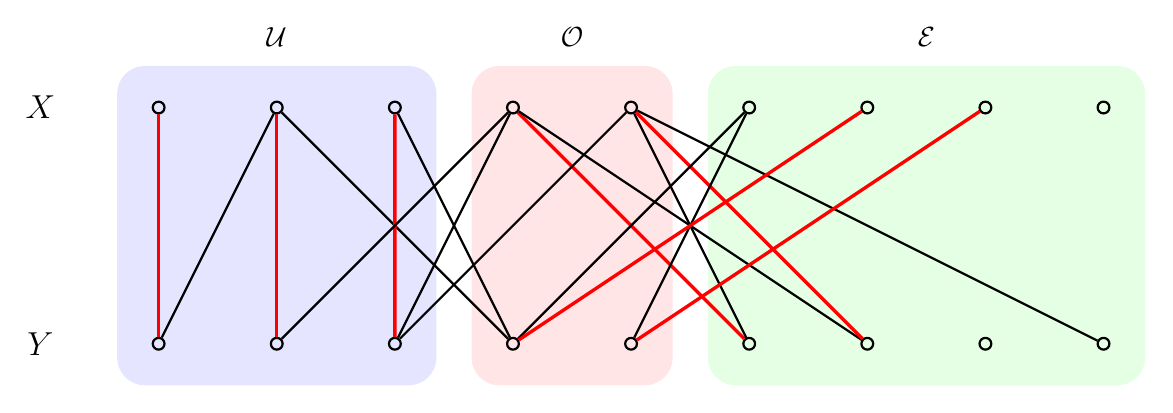
\begin{tikzpicture}[
    xscale=1.5, yscale=1.5, thick,
    every node/.style={draw, circle, inner sep=-1.5pt},
]

    \foreach \i in {1,...,9} {
        \node (x\i) at (\i, 2) {};
    }

    \foreach \i in {1,...,9} {
        \node (y\i) at (\i, 0) {};
    }

    \begin{scope}[on background layer]
        \draw[rounded corners=10pt, draw=none, fill=blue!10!white]
            ($(y1) - (10pt,10pt)$) rectangle ($(x3) + (10pt,10pt)$);
        \draw[rounded corners=10pt, draw=none, fill=red!10!white] 
            ($(y4) - (10pt,10pt)$) rectangle ($(x5) + (10pt,10pt)$);
        \draw[rounded corners=10pt, draw=none, fill=green!10!white] 
            ($(y6) - (10pt,10pt)$) rectangle ($(x9) + (10pt,10pt)$);
    \end{scope}

    \node[draw=none] at ($ (x1)!0.5!(x3) + (0,0.6) $) {$\mathcal U$};
    \node[draw=none] at ($ (x4)!0.5!(x5) + (0,0.6) $) {$\mathcal O$};
    \node[draw=none] at ($ (x6)!0.5!(x9) + (0,0.6) $) {$\mathcal E$};

    
    \draw (x1) -- (y1) [red, very thick];
    \draw (x2) -- (y1);
    \draw (x2) -- (y2) [red, very thick];
    \draw (x2) -- (y4);
    \draw (x3) -- (y3) [red, very thick];
    \draw (x3) -- (y4);
    \draw (x4) -- (y2);
    \draw (x4) -- (y3);
    \draw (x4) -- (y6) [red, very thick];
    \draw (x4) -- (y7);
    \draw (x5) -- (y3);
    \draw (x5) -- (y6);
    \draw (x5) -- (y9);
    \draw (x5) -- (y7) [red, very thick];
    \draw (x6) -- (y4);
    \draw (x6) -- (y5);
    \draw (x7) -- (y4) [red, very thick];
    \draw (x8) -- (y5) [red, very thick];

    \node[draw=none] at (0,2) {\large $X$};
    \node[draw=none] at (0,0) {\large $Y$};

\end{tikzpicture}
\end{document}
